\documentclass{beamer}

\usepackage[utf8]{inputenc}
\usepackage[T1]{fontenc} % Agregado para un mejor manejo de tipos en español
\usepackage[spanish]{babel}
\usepackage{amsmath}
\usepackage[nosetup]{evan}
\usetheme{Goddard}
\hypersetup{colorlinks,allcolors=.,urlcolor=magenta}
\usepackage[table]{xcolor} % Para definir colores en tablas
\usepackage{graphicx} % Para redimensionar la tabla
\title{Investigación de Operaciones I}
\subtitle{Unidad 1: Elementos de Programación Lineal}
\author{Ricardo Jesús Largaespada Fernández}
\institute{Ingeniería de Sistemas, DACTIC, UNI}
\date{11 de Agosto, 2025}

\begin{document}

\frame{\titlepage}

\begin{frame}
\frametitle{Agenda}
\tableofcontents
\end{frame}

\section{Datos Generales}
\begin{frame}
\frametitle{Datos del Curso}
\begin{itemize}
    \item \textbf{Asignatura}: Investigación de Operaciones I
    \item \textbf{Créditos}: 3
    \item \textbf{Frecuencia Semanal}: 2 sesiones
    \item \textbf{Semestre Académico}: Segundo Semestre 2025
    \item \textbf{Carrera}: Ingeniería de Sistemas
    \item \textbf{Horario de Atención}: L y Ma: 2M | L y Ma: 3M | L y Vi: 1M
    \item \textbf{Grupos}: 3M1-SIS-S | 3M2-SIS-S | 3M3-SIS-S
\end{itemize}
\end{frame}

\section{Objetivo General}
\begin{frame}
\frametitle{Objetivo General de la Asignatura}
\begin{itemize}
    \item Modelar problemas ingenieriles mediante Programación Lineal, que permiten obtener soluciones óptimas, para la interpretación de los resultados en la toma de decisiones.
\end{itemize}
\end{frame}

\section{Plan Temático}

\begin{frame}
\frametitle{Plan Temático}
\begin{center}
    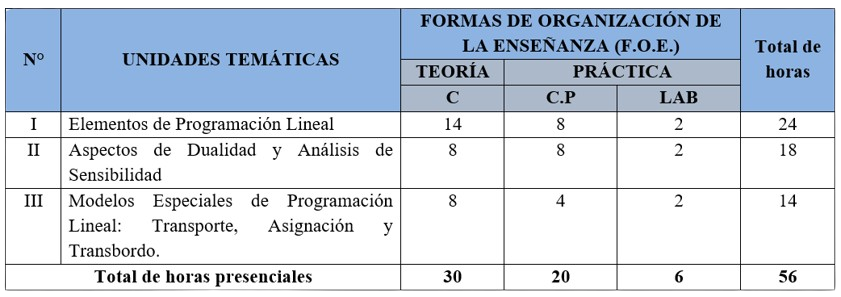
\includegraphics[scale=.3]{images/plan_tematico.png}
\end{center}
\end{frame}

\section{Unidad 1: Elementos de Programación Lineal}
\begin{frame}
\frametitle{Objetivos de la Unidad 1}
\begin{itemize}
    \item \textbf{Conceptual}: Identificar un problema de Programación Lineal, evaluando si sus componentes cumplen con todas las propiedades matemáticas necesarias distinguiendo entre las formas estándar y no estándar.
    \item \textbf{Procedimental}: Resolver un modelo de Programación Lineal, utilizando el método simplex y sus distintas variantes para clasificar el tipo de solución o soluciones en caso de que éstas existan.
    \item \textbf{Actitudinal}: Compartir la solución de diferentes problemas planteados como Programas Lineales para el análisis de la validez y las posibles formas de implementar dicha solución en la vida real.
\end{itemize}
\end{frame}

\section{Sesión 1}
\begin{frame}
\frametitle{Objetivos de la Sesión 1}
\begin{itemize}
    \item Identificar y diferenciar los elementos fundamentales de un problema de programación lineal, como son las variables de decisión, la función objetivo y las restricciones.
\end{itemize}
\end{frame}

\subsection{Optimización Matemática}
\begin{frame}
\frametitle{¿Qué es la optimización matemática?}
La optimización matemática es un término amplio que describe una forma de formular matemáticamente problemas de decisión y luego resolverlos utilizando algoritmos dedicados. 
\begin{block}{Nota}
Se usa en ingeniería, economía, logística, planificación de recursos, etc.
\end{block}
\end{frame}

\begin{frame}
\frametitle{Componentes de un modelo de optimización}
\begin{itemize}
    \item \textbf{Variables de decisión}: Correspondientes a acciones o elecciones en el problema.
    \item \textbf{Función objetivo}: Evalúa una solución específica, con un objetivo de maximización o minimización.
    \item \textbf{Restricciones}: Limitan los valores posibles de las variables de decisión.
\end{itemize}
\end{frame}

\begin{frame}
\frametitle{Región Factible}
Las restricciones definen la \textbf{región factible} de un modelo, es decir, el conjunto de todas las soluciones candidatas que cumplen con las restricciones.
\begin{block}{Recordatorio}
Si la región factible es vacía, no existe solución.
\end{block}
\end{frame}

\begin{frame}
\frametitle{Objetivo de un Modelo de Optimización}
El objetivo de un modelo de optimización es encontrar la mejor solución -- el \textbf{óptimo global} -- entre los valores de las variables de decisión que cumplen con todas las restricciones.
\end{frame}

\begin{frame}
\frametitle{Habilidades necesarias para la optimización matemática aplicada}
\begin{itemize}
    \item \textbf{¿Qué modelar?}
    \item \textbf{¿Cómo modelar?}
    \item \textbf{¿Cómo interpretar la solución del modelo?}
\end{itemize}
\end{frame}

\begin{frame}
\frametitle{Proceso Continuo en la Optimización}
Estos tres aspectos deben tratarse como un proceso continuo, no como pasos secuenciales.
\end{frame}

\begin{frame}
\frametitle{Descripción matemática de problemas de optimización}
Matemáticamente, podemos describir los problemas de optimización como sigue:

\begin{align*}
\min \quad &f(x)  \\
\text{sujeto a} \quad & x \in X,
\end{align*}
\end{frame}

\begin{frame}
\frametitle{Problemas de Maximización}
De manera similar, podemos definir un \textbf{problema de maximización} cambiando la condición final.
\end{frame}

\begin{frame}
\frametitle{Ejemplo y Tutorial}
En esta clase introductoria, presentamos un ejemplo simple de optimización en el contexto de la \textbf{planificación de la producción}.
\end{frame}

\begin{frame}
\frametitle{Enunciado del Problema}
Una empresa produce dos versiones de un producto. Cada versión se fabrica a partir de la misma materia prima que cuesta \$10 por gramo.
\begin{itemize}
    \item \textbf{Versión U}: Precio \$270, 10 g de materia prima, 1 hr de mano de obra A, 2 hrs de mano de obra B. Demanda $\leq$ 40 unidades/semana.
    \item \textbf{Versión V}: Precio \$210, 9 g de materia prima, 1 hr de mano de obra A, 1 hr de mano de obra B. Demanda ilimitada.
\end{itemize}
\end{frame}

\begin{frame}
\frametitle{Resumen de Datos}
\centering
\resizebox{0.85\textwidth}{!}{
\begin{tabular}{|c|c|c|c|c|c|}
\hline
\textbf{Versión} & \textbf{Materia Prima} & \textbf{Mano de Obra A} & \textbf{Mano de Obra B} & \textbf{Demanda del Mercado} & \textbf{Precio} \\
\hline
U & 10 g & 1 hr & 2 hr & $\leq$ 40 unidades & \$270 \\
\hline
V & 9 g & 1 hr & 1 hr & ilimitada & \$210 \\
\hline
\end{tabular}}

\centering
\begin{tabular}{|c|c|c|}
\hline
\textbf{Recurso} & \textbf{Cantidad Disponible} & \textbf{Costo} \\
\hline
Materia Prima & ? & \$10 / g \\
\hline
Mano de Obra A & 80 horas & \$50 / hora \\
\hline
Mano de Obra B & 100 horas & \$40 / hora \\
\hline
\end{tabular}
\end{frame}

\begin{frame}
\frametitle{Objetivo de la Empresa}
La empresa desea maximizar los beneficios brutos.

\begin{itemize}
    \item ¿Cuánta materia prima debería pedirse con anticipación para cada semana?
    \item ¿Cuántas unidades de $U$ y $V$ debería producir la empresa cada semana?
\end{itemize}
\end{frame}

\begin{frame}
\frametitle{Modelo Matemático}
El problema descrito anteriormente es un problema de optimización que incluye:
\begin{itemize}
    \item Variables de decisión
    \item Función objetivo
    \item Restricciones
\end{itemize}

\centering
\resizebox{0.85\textwidth}{!}{
\begin{tabular}{|c|l|c|c|}
\hline
\textbf{Variable de Decisión} & \textbf{Descripción} & \textbf{Límite Inferior} & \textbf{Límite Superior} \\
\hline
$x_M$ & Cantidad de materia prima utilizada & 0 & - \\
\hline
$x_A$ & Cantidad de Mano de Obra A utilizada & 0 & 80 \\
\hline
$x_B$ & Cantidad de Mano de Obra B utilizada & 0 & 100 \\
\hline
$y_U$ & Número de unidades de $U$ a producir & 0 & 40 \\
\hline
$y_V$ & Número de unidades de $V$ a producir & 0 & - \\
\hline
\end{tabular}}
\end{frame}

\begin{frame}
\frametitle{Función Objetivo}
El beneficio es igual a la diferencia entre los ingresos totales y el costo total de las operaciones:
$$
\text{beneficio} = \text{ingresos} - \text{costos}
$$
$$
\text{ingresos} = 270 y_U + 210 y_V
$$
$$
\text{costos} = 10 x_M + 50 x_A + 40 x_B
$$
$$
\text{maximizar} \quad 270 y_U + 210 y_V - 10 x_M - 50 x_A - 40 x_B
$$
\end{frame}

\begin{frame}
\frametitle{Restricciones}
$$
\begin{aligned}
    10 y_U + 9 y_V &\leq x_M \quad \text{(materia prima)} \\
    y_U + y_V &\leq x_A \quad \text{(mano de obra A)} \\
    2 y_U + y_V &\leq x_B \quad \text{(mano de obra B)} \\
\end{aligned}
$$
\end{frame}

\begin{frame}
\frametitle{Formulación del Problema Completo}
$$
\begin{align}
\text{maximizar} \quad & 270 y_U + 210 y_V - 10 x_M - 50 x_A - 40 x_B \\
\text{sujeto a} \quad & 10 y_U + 9 y_V \leq x_M \nonumber \\
 & 1 y_U + 1 y_V \leq x_A \nonumber \\
 & 2 y_U + 1 y_V \leq x_B \nonumber \\
 & 0 \leq x_M \nonumber \\
 & 0 \leq x_A \leq 80 \nonumber \\
 & 0 \leq x_B \leq 100 \nonumber \\
 & 0 \leq y_U \leq 40 \nonumber \\
 & 0 \leq y_V. \nonumber
\end{align}
$$
\end{frame}

\begin{frame}
\frametitle{Solución Óptima}
Una solución óptima es cualquier asignación de valores a las variables de decisión que cumpla con las restricciones y que maximice o minimice el objetivo.
\end{frame}

\begin{frame}
\frametitle{Algoritmos de Optimización}
Los algoritmos de optimización matemática son procedimientos genéricos que pueden encontrar soluciones óptimas siempre que los problemas se formulen de manera estandarizada.\\

Para los profesionales, la optimización matemática a menudo implica formular el problema como un modelo y luego pasarlo a un paquete de software especializado.
\end{frame}

\begin{frame}
\frametitle{Solución Óptima - Ejemplo Numérico}
Suponiendo que resolvemos el modelo con método símplex:
\pause
\begin{itemize}
    \item $y_U = 20$ unidades \pause
    \item $y_V = 60$ unidades \pause
    \item $x_M = 10(20) + 9(60) = 740$ g \pause
    \item Beneficio máximo: \$15\,900
\end{itemize}
\pause
\begin{block}{Interpretación}
Es óptimo producir ambas versiones en las cantidades calculadas para usar eficientemente los recursos y maximizar el beneficio.
\end{block}
\end{frame}

\begin{frame}
\frametitle{Preguntas}
\centering
\Huge{¿Preguntas?}
\end{frame}

\end{document}
